% Chapter 1
\chapter{مقدمه}
در سال‌های اخیر با توجه به افزایش چشم گیر استفاده از شبکه های کامپیوتری و نیازمندی این شبکه ها به دینامیک بالا به منظور اعمال تغییرات و برنامه ریزی سریع، مفهوم نسبتا جدیدی به نام شبکه های تعریف شده بر مبنای نرم افزار یا \lr{SDN} پدید آمده است.

\section{شبکه نرم افزار محور (\lr{SDN})}
شبکه های نرم افزار محور (\lr{SDN}) مفهوم نو ظهوری در شبکه‌های کامپیوتری است که برمبنای آن کنترل کننده‌های منطقی مجتمع، رفتار شبکه را کنترل می‌کنند. این گونه از معماری شبکه، فرصت‌های جدیدی به منظور ایجاد دینامیک بالاتر و تغییرات آنی و همچنین پیاده سازی مدل های مختلف امنیت را فراهم می‌آورد.\\
در این معماری، بخش کنترل کننده\LTRfootnote{Control Plane} تجهیزات از بخش هدایت کننده داده‌ها\LTRfootnote{Data Plane} جدا شده و این امر موجب فراهم آوردن بستری به منظور برنامه ریزی مستقیم شبکه از طریق نرم افزار و انتزاعی ساختن زیرساخت شبکه از دید برنامه‌ها و سرویس‌های شبکه شده است.

\begin{figure}
	\centering
	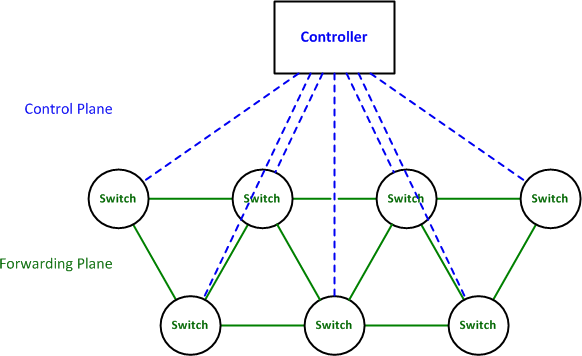
\includegraphics[scale=0.5]{imgs/SDN_controller.png}
	\caption{نمایی انتزاعی از معماری شبکه های نرم افزار محور}
	\label{fig1}
\end{figure}

\section{مزایای معماری \lr{SDN}}


\begin{itemize}
	\item
قابلیت برنامه ریزی مستقیم: با توجه به پیاده سازی بخش منطق و تصمیم‌گیری تجهیزات به صورت مجزا و در بستر نرم‌افزار، امکان برنامه ریزی مستقیم هر یک از بخش‌های شبکه از طریق رابط‌های نرم‌افزاری وجود دارد.
	\item 
دینامیک بالا و تغییرات لحظه‌ای: همانظور که انتظار می‌رود با پیشرفت استفاده از شبکه‌ها، نیازمندی به تغییرات آنی در ساختار شبکه بیش از پیش احساس می‌گردد. با توجه به قابلیت برنامه ریزی مستقیم تجهیزات می‌توان توسط رابط های نرم‌افزاری، تنظیمات و مسیر‌های حرکت داده را به صورت خودکار و آنی تغییر داد.
	\item 
مدیریت متمرکز: با جداسازی بخش تصمیم گیرنده از بخش هدایت داده، می‌توان تجهیزات را به صورت متمرکز کنترل کرد. اما این مزیت خود یک عیب بزرگ نیز به شمار می‌رود. درصورتی که کنترل کننده مرکزی به هر دلیلی از دسترس خارج شود،‌تمام شبکه از کار خواهد افتاد. راه حل این مشکل، پیاده سازی دسته‌ای\LTRfootnote{Cluster} از کنترل کننده‌ها به منظور ایجاد قابلیت اطمینان در شبکه است.
	\item
پایداری بالا: پایداری بالا، یکی از عوامل اصلی در اطمینان از عملکرد مناسب و مداوم شبکه است. با وجود قابلیت‌هایی نظیر تغییرات آنی و مدیریت مرکزی، شبکه‌های مبتنی بر نرم‌افزار قادر تشخیص هرگونه اشکال و ناهماهنگی در سطح شبکه و رفع سریع آن با پیدا کردن مسیر‌های جایگزین هستند.
	\item 
اختصاصی نبودن نرم افزار و سیستم عامل‌های شبکه (مبتنی بر استاندارد‌های آزاد و عدم وابستگی به فروشنده تجهیز شبکه): در شبکه‌های سنتی زمانی که از تجهیزات برند‌های مختلف استفاده می‌شد، نرم‌افزار و سیستم عامل‌های آن نیز اختصاص به همان برند خاص داشت و این باعث مختلف شدن پیکربندی‌های یکسان در برند‌های متفاوت می‌شد. با ظهور پدیده شبکه‌های مبتنی بر نرم‌افزار، این مرز بین برند‌ها برداشته شده و تمام تجهیزات با زبانی مشترک قابل پیکربندی می‌باشد.
\end{itemize}

\section{اجزاء تشکیل دهنده معماری \lr{SDN}}
با توجه به شکل \ref{fig2} یک شبکه مبتنی بر نرم‌افزار از اجزاء مختلفی تشکیل شده است که در ادامه به شرح وظایف هر یک از بخش‌ها می‌پردازیم.
\begin{figure}
	\centering
	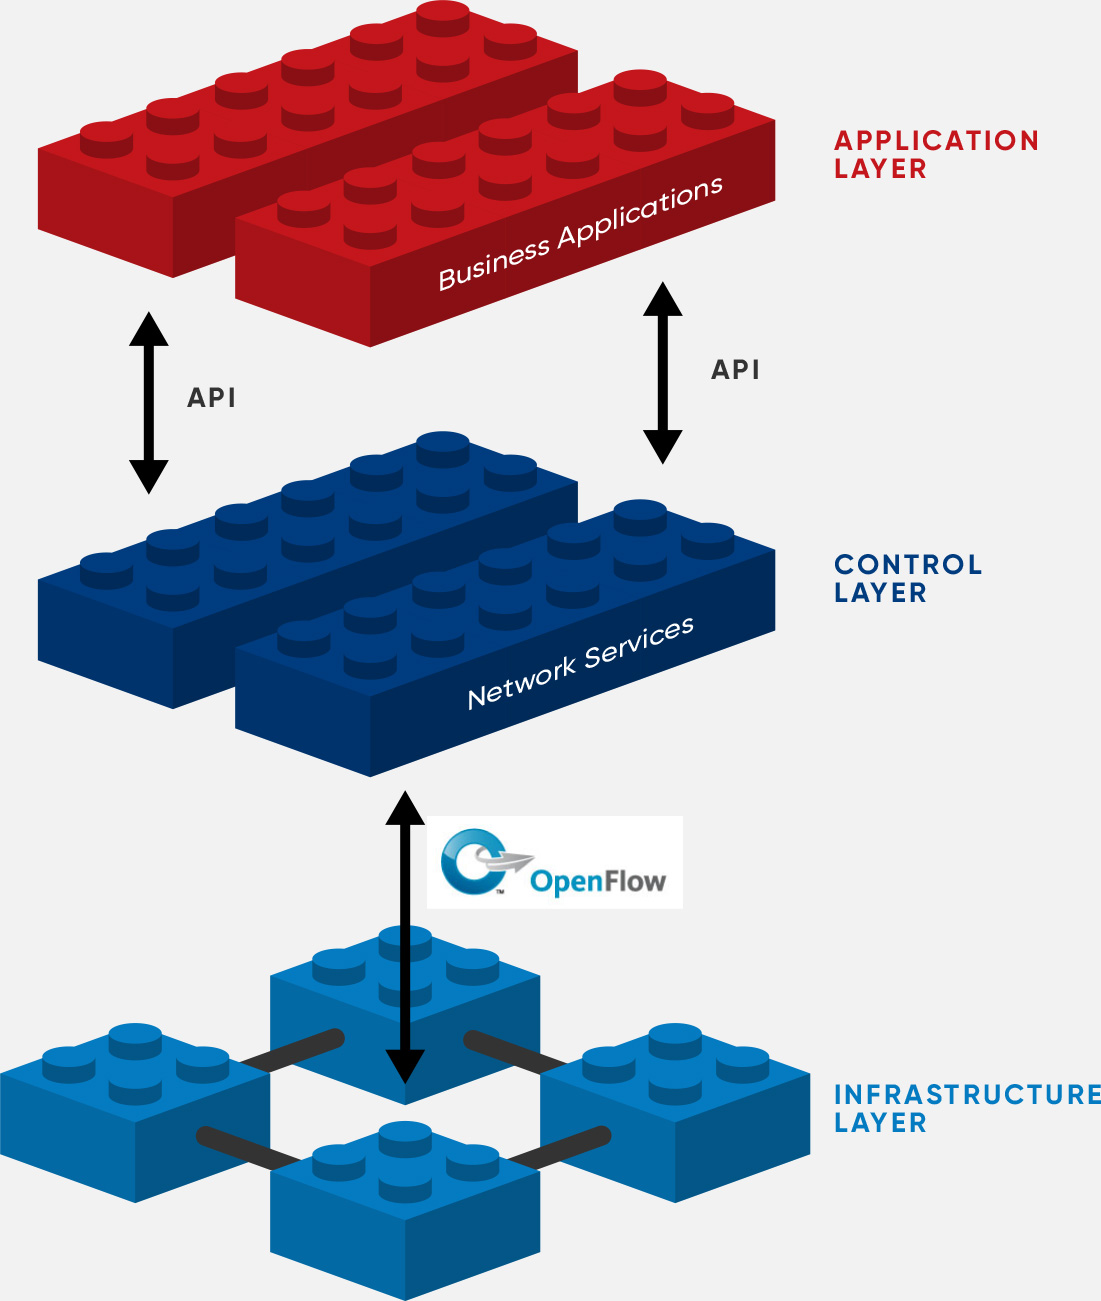
\includegraphics[scale=0.2]{imgs/sdn-architecture-img.jpg}
	\caption{نمایی از اجزاء تشکیل دهنده شبکه های مبتنی بر نرم‌افزار}
	\label{fig2}
\end{figure}

\subsection{لایه زیرساخت}
لایه زیرساخت\LTRfootnote{ّInfrastructure Layer}، مجموعه‌ای از تجهیزات شبکه مانند سوئیچ‌ها ،مسیریاب‌ها و سرور‌ها هستند که وظیفه هدایت ترافیک شبکه را عهده دار می‌باشند. این لایه درواقع لایه فیزیکی کنترل شده توسط کنترل کننده‌های \lr{SDN} است.

\subsection{ارتباط جنوبی}
ارتباط جنوبی\LTRfootnote{SouthBound Interface (SBI)} که بین لایه زیرساخت و لایه کنترل قرار دارد یکی از مهم‌ترین بخش‌های معماری \lr{SDN} می‌باشد. از جمله پروتکل‌‌ها در این ارتباط می‌توان به \lr{OpenFlow} ، \lr{Netconf} و \lr{OVSDB} اشاره کرد. ما در این پروژه به بررسی اجمالی پروتکل \lr{OpenFlow} و قابلیت‌های نسخه‌ی جدید آن می‌پردازیم.

\subsection{لایه کنترل}
لایه کنترل\LTRfootnote{Control Layer} در واقع هسته اصلی تصمیم گیری‌های شبکه و مغز متفکر آن می‌باشد. بخش اعظم فعالیت شرکت‌های تولید کننده‌ راهکار‌های شبکه‌ مبتنی بر نرم‌افزار، اختصاص به ساخت و توسعه کنترل کننده‌ها و بستر‌های نرم افزاری این لایه دارد. در این لایه، وظیفه مهم تصمیم گیری نحوه هدایت بسته‌ها، جمع‌آوری اطلاعات شبکه، وضعیت هر یک از بخش‌ها، جزئیات توپولوژی، وضعیت آماری بخش مختلف و غیره با برنامه ریزی لایه زیرساخت توسط ارتباط جنوبی انجام می‌شود.

\subsection{ارتباط شمالی}
ارتباط شمالی\LTRfootnote{NorthBound Interface (NBI)} که بین لایه کنترل و لایه برنامه کاربردی قرار دارد، وظیفه ایجاد بستر ارتباطی به منظور برنامه ریزی کنترل کننده را به عهده دارد. از جمله مهم ترین پروتکل‌های ارتباط شمالی میتوان به \lr{REST API} اشاره نمود.

\subsection{لایه برنامه کاربردی}
لایه برنامه کاربردی\LTRfootnote{Application Layer}، محلی برای اجرای برنامه‌های کاربردی است. این برنامه‌ها با استفاده از اطلاعاتی که از لایه کنترل کننده به آن‌ها داده می‌شود اقدام به ایجاد تغییرات در شبکه و مسیر‌ها می‌کنند. از نمونه‌های این برنامه‌ها می‌توان به اتوماسیون شبکه\LTRfootnote{Network Automation}، مدیر و پیکربندی شبکه\LTRfootnote{Network Configuration and Management}، پایش وضعیت شبکه\LTRfootnote{Network Monitoring}، عیب یابی شبکه\LTRfootnote{Network Troubleshooting} و امنیت شبکه\LTRfootnote{Network Security} اشاره کرد.

\section{نحوه عملکرد و تفاوت آن با شبکه‌های سنتی}

\begin{figure}
	\centering
	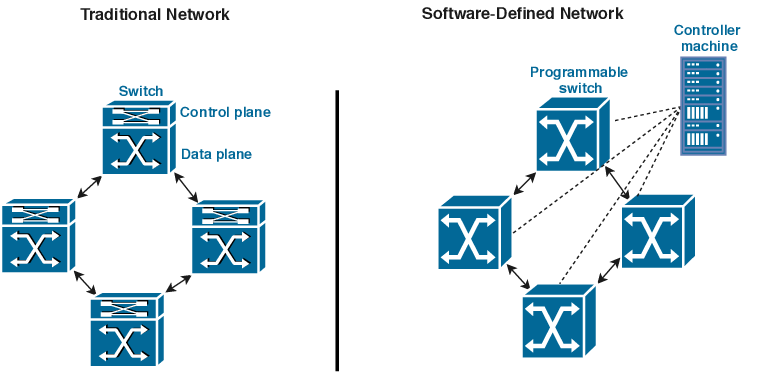
\includegraphics[scale=0.3]{imgs/sdn_vs_trad.png}
	\caption{تفاوت شبکه مبتنی بر نرم‌افزار با شبکه سنتی}
	\label{fig3}
\end{figure}

با توجه به شکل \ref{fig3}، در شبکه‌های سنتی، هر تجهیز دارای بخش منطق و تصمیم گیری بوده و با دریافت اطلاعات هر یک از تجهیزات دیگر، اقدام به هدایت داده‌ها می‌کند اما در معماری مدرن \lr{SDN}، هر یک از تجهیزات ابتدا بسته‌ها را به سمت کنترل به منظور تصمیم گیری هدایت می‌کنند، سپس کنترل کننده با توجه به قواعد تعیین شده و ایجاد تطابق با آن‌ها، یک جریان\LTRfootnote{Flow} تشکیل داده و آن را به بخش هدایت داده ارسال می‌کند، پس از آن هربار که تجهیز بسته مشابهی دریافت کرد آن را با توجه به جریان موجود در جدول جریان\LTRfootnote{Flow Table} هدایت می‌کند.

\section{ساختار گزارش}
در این گزارش هدف، بررسی ویژگی‌های جدید پروتکل \lr{Openflow} است. در فصل اول توضیحات جامعی در مورد پروتکل \lr{Openflow} و نحوه عملکرد آن در معماری \lr{SDN} داده می‌شود. سپس در فصل دوم ویژگی‌های اضافه شده به نسخه‌ \lr{OF1.5} مورد بررسی قرار می‌گیرد .





